\begin{figure}[ht]
    \centering
    \caption{Desempenho CLF\underscore{}ACC da solução reproduzida para o corpus DB\underscore{}AUTHORPROF.}
    \vspace{-0.5cm}
    \begin{center}
        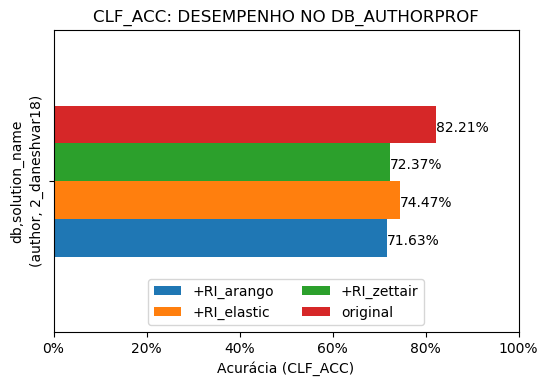
\includegraphics[scale=0.75]{img/clf-acc-bars-authorprof.png}
    \end{center}
    \vspace{-0.5cm}
    \legend{\ABNTEXfontereduzida \textbf{Fonte:} O autor.}
    \label{fig:clf-acc-bars-authorprof}
\end{figure}